%-------------------------------------------------------------------------------
% CAPITOLO 21
%-------------------------------------------------------------------------------
\chapter{Lezione 21}
\label{capitolo_21}
\textit{16/05/2026}

\section{Modello della Membrana Neuronale}
Modelliamo la membrana di un neurone come un condensatore. Sulla membrana sono presenti diversi tipi di canali ionici.
L'equazione che descrive la variazione del potenziale di membrana $V$ nel tempo è data da:

\begin{equation} \label{eq:ch21_1}
C\frac{dV}{dt} = \sum_{i}^{N_{ch}} g_{i}N_{i}f_{i}(V_{i}-V) + I_{ext}
\end{equation}

dove:
\begin{itemize}
    \item $C$ è la capacità della membrana.
    \item $i$ è un indice che specifica il tipo di canale ionico considerato.
    \item $g_i$ è la conduttanza del singolo canale di tipo $i$.
    \item $N_i$ è il numero totale di canali di tipo $i$.
    \item $f_i$ è la frazione di canali di tipo $i$ che sono aperti.
    \item $V_i$ è il potenziale di riposo per quel tipo di canale, ovvero il valore che il potenziale di membrana dovrebbe avere affinché in quello specifico canale non ci sia corrente.
    \item $V$ è la differenza di potenziale attraverso l'intera membrana, determinata da tutti i tipi di canali.
    \item $I_{ext}$ è un contributo esterno alla corrente, ad esempio proveniente da altri neuroni.
\end{itemize}

La dinamica della frazione di canali aperti $f_i$ è descritta da un'equazione di rilassamento:

\begin{equation} \label{eq:ch21_2}
\frac{df_i}{dt} = -\frac{1}{\tau_i}(f_i - f_i^{eq}(V))
\end{equation}

dove $\tau_i$ è la costante di tempo caratteristica del canale $i$ e $f_i^{eq}(V)$ è la frazione di canali aperti all'equilibrio, che dipende dal potenziale di membrana $V$.
L'espressione esplicita di $f_i^{eq}(V)$ può essere derivata da un modello a due stati:

\begin{equation} \label{eq:ch21_3}
f_i^{eq}(V) = \frac{1}{1 + \exp\left(\frac{V-V_{1/2}}{\Delta}\right)}
\end{equation}

dove $V_{1/2}$ è il potenziale al quale metà dei canali sono aperti e $\Delta$ caratterizza la sensibilità al voltaggio. La varianza $\Delta$ è data dalla carica che si muove dall'interno all'esterno della membrana se il canale si apre.

\subsection*{Feedback positivo}
Consideriamo lo stato stazionario del sistema, che chiamiamo $V_0$. Si analizza cosa succede se si perturba lo stato stazionario $V_0$ con una piccola perturbazione $\delta V$.
Linearizzando il sistema di equazioni, si osserva che esiste una classe di canali veloci che contribuisce con una sorta di resistenza negativa, facilitando il passaggio attraverso la membrana.
Questi canali soddisfano le seguenti condizioni:

\textbf{Prima condizione:}
\begin{equation} \label{eq:ch21_4}
f_i^{eq}(V_0) > 0 
\end{equation}

La prima condizione implica che, anche allo stato stazionario (o di riposo) $V_0$, una frazione seppur piccola di questi canali ionici di tipo $i$ è già aperta. Questo è importante perché implica che i canali sono pronti a rispondere a variazioni di potenziale; non sono in uno stato completamente "chiuso" o inattivo dal quale sarebbe più difficile "attivarli". Se $f_i^{eq}(V_0)$ fosse nulla, una piccola depolarizzazione potrebbe non essere sufficiente ad innescare la loro apertura.

\textbf{Seconda condizione:}
\begin{equation} \label{eq:ch21_5}
\left. \frac{df_i^{eq}}{dV}\right|_{V_0} > 0 
\end{equation}

La seconda condizione indica che la frazione di canali di tipo $i$ aperti all'equilibrio aumenta all'aumentare del potenziale di membrana $V$ (cioè, quando la membrana si depolarizza a partire da $V_0$). Una piccola depolarizzazione della membrana, quindi, causerà l'apertura di un numero maggiore di questi canali.

L'effetto combinato di queste due condizioni fa sì che i canali facilitano il passaggio della corrente attraverso la membrana. Ciò indica che i canali forniscono un feedback positivo alla membrana: se il potenziale aumenta rispetto al valore di equilibrio, l'aumento del potenziale innesca l'apertura di questi canali, e l'apertura dei canali spinge il potenziale a un valore maggiore, che innesca l'apertura di ulteriori canali, e così via. Questo spiega l'apertura improvvisa di molti canali e perché il potenziale di membrana cambia molto rapidamente, portando al cosiddetto potenziale d'azione.


\section{Caso Semplificato con Due Tipi di Canali}
Consideriamo un caso semplice con solo due tipi di canali:
\begin{itemize}
    \item \textbf{Canali di leak:} questi canali sono sempre aperti. La loro frazione di apertura è costante e uguale a 1. Si assume un potenziale di inversione $V_i = V_{leak} = 0$ e la loro conduttanza totale è $G_L = g_{\text{leak}}N_{\text{leak}}$.
    \item \textbf{Altri canali (canali attivi):} questi canali sono tutti uguali, con un potenziale di riposo $V_i = V_R$. La loro conduttanza totale è $g \cdot N$, dove $g$ è la conduttanza del singolo canale attivo e $N$ il loro numero totale. Questi sono i canali responsabili del feedback positivo e la loro frazione di apertura dipende dal voltaggio secondo l'equazione:
\end{itemize}

\begin{equation} \label{eq:ch21_6}
\frac{df}{dt} = -\frac{1}{\tau}(f - f^{eq}(V))
\end{equation}

Abbiamo omesso l'indice $i$ poiché c'è solo un tipo di canale attivo.
In questo caso, l'equazione per il potenziale di membrana diventa:

\begin{equation} \label{eq:ch21_7}
C\frac{dV}{dt} = -G_L V + gNf(V_R - V) + I_{ext}
\end{equation}

\subsection*{Stato Stazionario}
Per trovare lo stato stazionario, poniamo le derivate temporali a zero ($dV/dt = 0$ e $df/dt = 0$).
Dall'equazione (\ref{eq:ch21_7}) (assumendo $I_{ext}=0$ per semplicità nello stato stazionario):

\begin{equation} \label{eq:ch21_8}
G_L V = gNf(V_R - V)
\end{equation}

Da cui possiamo esprimere $f$ in funzione di $V$:

\begin{equation} \label{eq:ch21_9}
f = \frac{G_L V}{gN(V_R - V)}
\end{equation}

Dall'equazione (\ref{eq:ch21_6}):

\begin{equation} \label{eq:ch21_10}
f = f^{eq}(V) = \frac{1}{1 + \exp\left(\frac{V-V_{1/2}}{\Delta}\right)}
\end{equation}

Possiamo risolvere graficamente questo sistema cercando le intersezioni delle due curve $f(V)$.

\begin{figure}[h!]
\centering
% 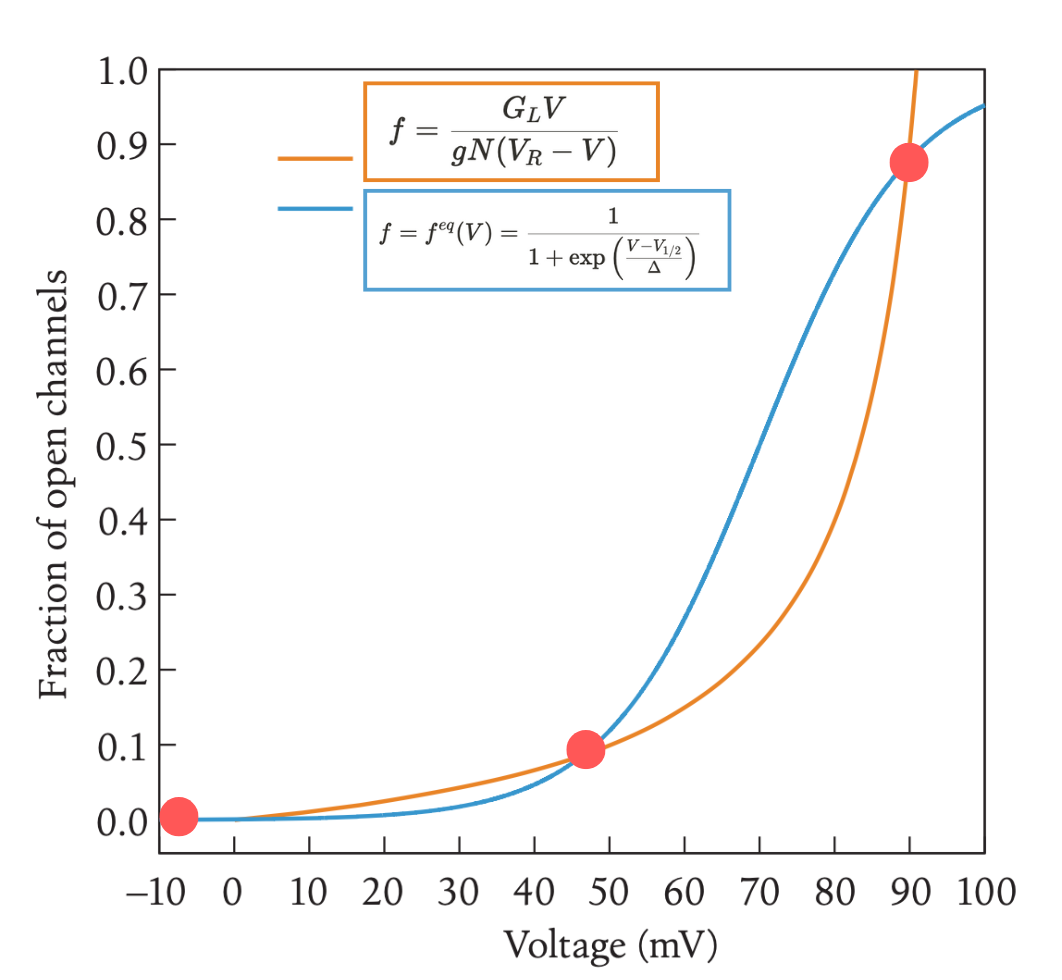
\includegraphics[width=0.6\textwidth]{pics/21_1.png} % INSERIRE QUI IL GRAFICO DELLE INTERSEZIONI DELLE CURVE f(V)
\caption{Risoluzione grafica per lo stato stazionario: intersezioni tra la curva di equilibrio $f^{eq}(V)$ e la curva derivata dalla condizione stazionaria del potenziale.}
\label{fig:ch21_1}
\end{figure}

Si ottengono tre soluzioni: due stabili e una instabile.
\begin{itemize}
    \item \textbf{Uno stato stabile a basso $V$ e basso $f$:} Questo corrisponde allo stato di riposo del neurone. Se il sistema si trova in prossimità di questo punto, piccole perturbazioni lo faranno ritornare a questo stato. In questo stato, la maggior parte dei canali è chiusa (fatta eccezione per quelli di leak).
    \item \textbf{Uno stato instabile a $V$ intermedio.}
    \item \textbf{Uno stato stabile ad alto $V$ e alto $f$:} Questo corrisponde allo stato eccitato del neurone, o al picco del potenziale d'azione, dove una frazione significativa dei canali attivi è aperta.
\end{itemize}

L'evoluzione del sistema è determinata in modo cruciale dalla posizione rispetto al punto di instabilità. Se un impulso di corrente esterna $I_{ext}$ è sufficientemente intenso da elevare il potenziale di membrana $V$ al di sopra del valore corrispondente al punto instabile, il sistema non ritorna più allo stato di riposo. Si attiva, invece, un processo evolutivo a cascata:

\begin{enumerate}
    \item Il nuovo valore di $V$, ora superiore alla soglia di instabilità, porta il sistema a cercare una nuova frazione di equilibrio di canali aperti $f$, come dettato dalla curva $f^{eq}(V)$. Questa frazione $f$ risulterà maggiore di quella associata al punto instabile.
    \item Questa maggiore frazione di canali aperti $f$, a sua volta, induce una variazione del potenziale di membrana $V$, che tenderà verso il valore imposto dalla relazione stazionaria $f(V)$. Questo nuovo valore di $V$ sarà ulteriormente incrementato.
    \item Tale sequenza iterativa, in cui lo stato del sistema si sposta alternativamente tra le condizioni imposte dalle due curve di stazionarietà, prosegue, spingendo progressivamente il sistema verso il secondo punto stabile, caratterizzato da un elevato potenziale $V$ e una grande frazione di canali attivi aperti.
\end{enumerate}

In caso contrario, se la perturbazione non supera la soglia di instabilità, il sistema ritorna allo stato di riposo iniziale.
Questa analisi grafica illustra in modo esplicito l'effetto di feedback positivo e come una perturbazione sopra soglia possa innescare il potenziale d'azione, portando il neurone dallo stato di riposo a quello eccitato.

\begin{figure}[h!]
\centering
% 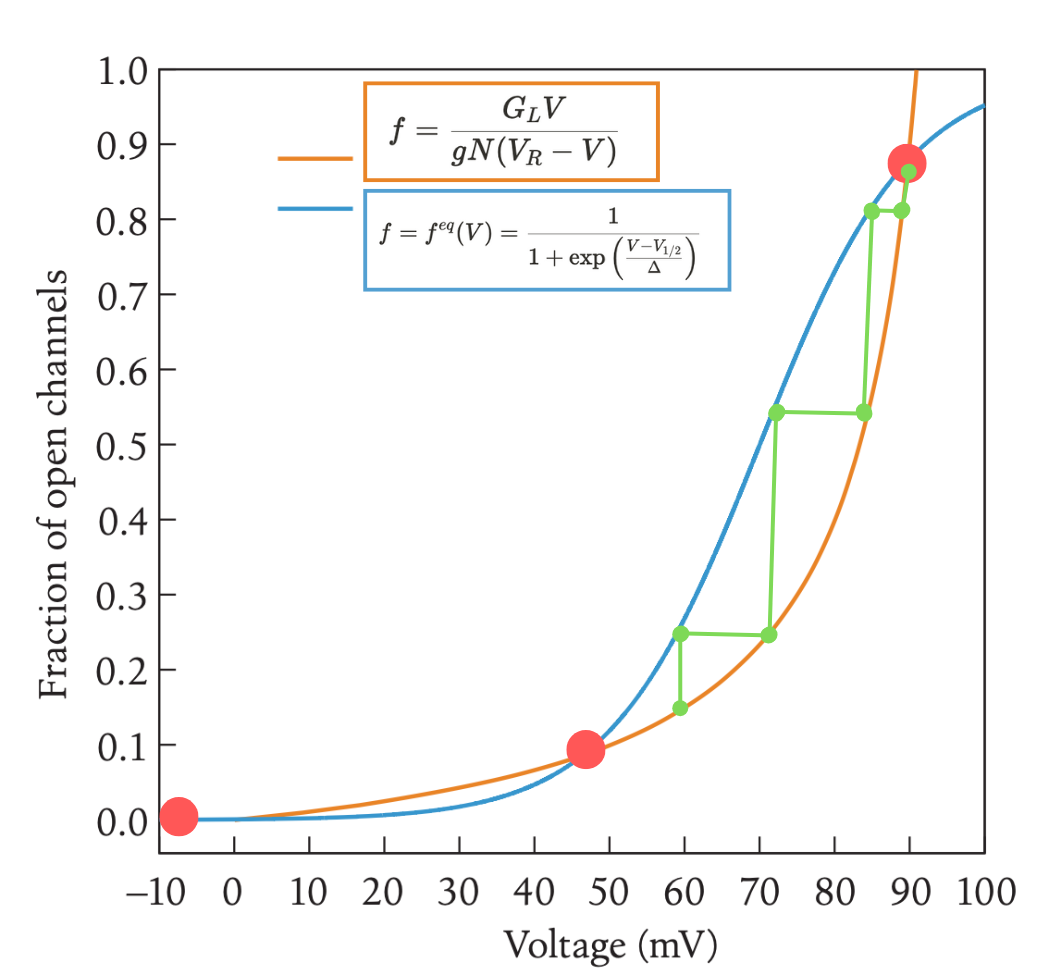
\includegraphics[width=0.6\textwidth]{pics/21_2.png} % INSERIRE QUI IL GRAFICO DELLE INTERSEZIONI DELLE CURVE f(V)
\caption{Effetto di feedback positivo.}
\label{fig:ch21_2}
\end{figure}

\section{Modelli Neuronali Più Realistici}
La descrizione precedente è semplificata. Modelli più realistici dei neuroni includono ulteriori complessità:
\begin{itemize}
    \item \textbf{Porte dei canali (gates):} Si assume che ogni canale abbia diversi gates (attivazione e inattivazione) e che il canale si apra solo quando tutti i gates rilevanti sono aperti. La frazione di canali aperti $f_i$ viene espressa in termini di frazioni di questi gates:
\end{itemize}

\begin{equation} \label{eq:ch21_11}
f_i = m_i^{\alpha_i} h_i^{\beta_i}
\end{equation}

dove $m_i$ è la frazione di gates di attivazione aperti e $h_i$ è la frazione di gates di inattivazione aperti. Per $m_i$ e $h_i$ si scrivono equazioni dinamiche simili a quella per $f_i$.

\begin{itemize}
    \item \textbf{Dipendenza spaziale del potenziale:} Il potenziale di membrana $V$ può variare non solo nel tempo ma anche lungo la posizione $z$ dell'assone del neurone.
\end{itemize}

\begin{equation} \label{eq:ch21_12}
V \equiv V(z,t)
\end{equation}

Includendo questi dettagli si ottengono le equazioni di Hodgkin-Huxley, che possono descrivere la propagazione degli impulsi lungo l'assone.


\section{Reti Neurali}
Dopo aver analizzato la dinamica del singolo neurone, che si caratterizza per processi di trasmissione del segnale molto rapidi, ci si concentra ora sul comportamento collettivo di molti neuroni interconnessi. L'idea di base è che un singolo neurone, in assenza di stimoli significativi, si trovi in uno stato di quiescenza (silente). Tuttavia, riceve continuamente segnali da numerosi altri neuroni con cui è connesso. Quando il segnale cumulativo in ingresso supera una certa soglia critica, il neurone si attiva e genera un potenziale d'azione.

Per modellare una rete di neuroni, si assegna a ciascun neurone $i$ una variabile binaria $S_i$:
\begin{itemize}
    \item $S_i = +1$: stato attivo.
    \item $S_i = -1$: stato silente.
\end{itemize}

L'idea è che un neurone $i$ si attivi se il segnale cumulativo che riceve dagli altri neuroni $S_j$ (pesato dalle connessioni sinaptiche $W_{ij}$) supera una soglia $\vartheta_i$:

\begin{equation} \label{eq:ch21_13}
S_i= \text{sgn}\left(\sum_j W_{ij}S_j- \vartheta_i\right)
\end{equation}

dove $\text{sgn}(x)$ è la funzione segno che restituisce $+1$ se $x > 0$ e $-1$ se $x < 0$.
I pesi sinaptici $W_{ij}$ codificano la forza dell'influenza del neurone $j$ sul neurone $i$. $W_{ij}$ può essere nullo se non c'è connessione diretta, oppure può assumere valori diversi indicanti connessioni più o meno forti, a seconda, ad esempio, del numero di contatti sinaptici tra l'assone di $j$ e i dendriti di $i$.
Questa equazione ricorda l'equazione di campo medio per il modello di Ising a temperatura zero.
L'equazione di campo medio per il modello di Ising è:

\begin{equation} \label{eq:ch21_14}
m_i = \tanh\left(\beta h_i + \beta J \sum_j M_{ij}m_j\right)
\end{equation}

dove $m_i$ è la magnetizzazione locale, $h_i$ il campo esterno locale, $J$ la costante di accoppiamento, $M_{ij}$ la matrice di interazione e $\beta = 1/(k_B T)$.
A temperatura $T \to 0$, la funzione tangente iperbolica $\tanh(\beta x)$ diventa una funzione a gradino, equivalente alla funzione segno $\text{sgn}(x)$; l'equazione (\ref{eq:ch21_14}) diventa:

\begin{equation} \label{eq:ch21_15}
m_i = \text{sgn} \left(\beta h_i + \beta J \sum_j M_{ij}m_j\right)
\end{equation}

Quindi, l'equazione per l'attivazione neuronale è analoga a un modello di Ising a $T=0$.
Questa analogia suggerisce che sia possibile definire una Hamiltoniana per la rete neurale, tale che gli stati stabili della dinamica neuronale corrispondano ai minimi di questa energia.
Per analogia con l'Hamiltoniana del modello di Ising, si può postulare un'Hamiltoniana per la rete neurale della forma:

\begin{equation} \label{eq:ch21_16}
H_N = -\frac{1}{2}\sum_{i, j} W_{ij}S_iS_j + \sum_i \vartheta_i S_i
\end{equation}


\section{Modellare la Memoria}
L'obiettivo primario nello studio di tali reti neurali è comprendere come possano immagazzinare e recuperare informazioni, ovvero come possano funzionare da memorie associative.
L'idea centrale è che la memoria corrisponda a un pattern specifico di attività neuronale, cioè una particolare configurazione degli stati $\{S_i\}$ dei neuroni della rete.
Indichiamo un pattern di memoria con $\{\xi_i^\mu\}$, dove $\xi_i^\mu = \pm 1$ per ogni neurone $i$, e $\mu$ è un indice che etichetta i diversi pattern memorizzati.
Il requisito fondamentale è che questi pattern di memoria siano stati stabili della dinamica della rete. Ciò significa che se la rete viene posta in una configurazione $\{S_i\}$ vicina a un pattern memorizzato, la sua evoluzione dinamica dovrebbe portarla a convergere precisamente a quel pattern (non ad un mix di due diversi pattern) e a rimanervi:

\begin{equation*}
\{S_i\} \longrightarrow  \{\xi_i^\mu\} 
\end{equation*}

In termini dell'analogia con i sistemi fisici, si desidera che i pattern di memoria $\{\xi_i^\mu\}$ corrispondano a minimi locali del landscape energetico definito dall'Hamiltoniana $H_N$.
La questione cruciale è come scegliere i pesi sinaptici $W_{ij}$ (e le soglie $\vartheta_i$, che per semplicità iniziale si pongono uguali a zero) affinché la rete esibisca i pattern desiderati come stati stabili.

\begin{itemize}
    \item \textbf{Modello di Ising ferromagnetico:} Una prima ipotesi, mutuata direttamente dal modello di Ising ferromagnetico, potrebbe essere quella di porre tutti i $W_{ij}$ uguali a una costante positiva $J$. Tuttavia, un tale sistema avrebbe solo due stati fondamentali stabili: quello con tutti i neuroni attivi ($S_i = +1$ per ogni $i$) e quello con tutti i neuroni silenti ($S_i = -1$ per ogni $i$). Questo limiterebbe drasticamente la capacità di memoria a soli due pattern molto specifici, il che è chiaramente insufficiente.
    \item \textbf{Modello di vetro di spin:} Un'alternativa opposta sarebbe scegliere i $W_{ij}$ in modo casuale. Questo porta a un modello noto come "spin glass" (vetro di spin). I vetri di spin sono caratterizzati da un fenomeno chiamato "frustrazione": a causa della natura disordinata e competitiva delle interazioni (alcune positive, altre negative), non è possibile soddisfare simultaneamente tutti i legami energetici.
\end{itemize}

Un semplice esempio di frustrazione si ha in un reticolo triangolare di spin con interazioni antiferromagnetiche: se due spin adiacenti sono anti-allineati per minimizzare la loro energia, il terzo spin non può soddisfare contemporaneamente il legame con entrambi.

\begin{figure}[h!]
\centering
% 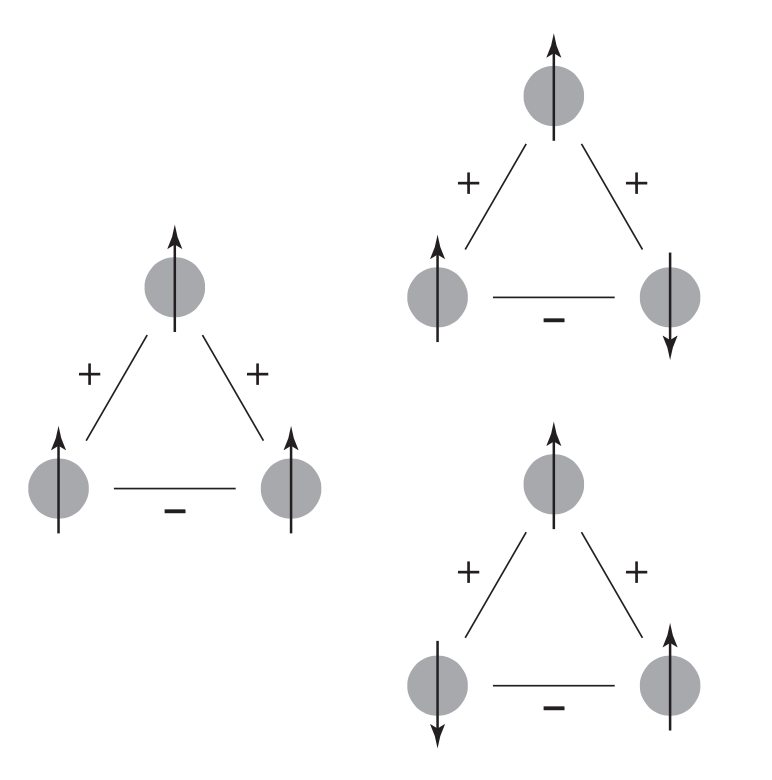
\includegraphics[width=0.4\textwidth]{pics/21_3.png} % INSERIRE QUI LO SCHEMA DELLA FRUSTRAZIONE (ES. TRIANGOLO ANTIFERROMAGNETICO)
\caption{Esempio di frustrazione in un reticolo triangolare con interazioni antiferromagnetiche.}
\label{fig:ch21_3}
\end{figure}

La conseguenza della frustrazione è un landscape energetico estremamente complesso, con un numero elevatissimo di minimi locali sub-ottimali, molti dei quali possono avere energie simili.
Se da un lato la presenza di molti minimi potrebbe sembrare vantaggiosa per immagazzinare numerosi pattern, i vetri di spin presentano un problema significativo: la posizione esatta di questi minimi nello spazio delle configurazioni è estremamente sensibile a piccole variazioni nei valori dei $W_{ij}$. Questa fragilità rende i vetri di spin inadatti come modello per una memoria robusta, poiché la perdita o l'alterazione di poche connessioni sinaptiche potrebbe stravolgere l'intera struttura delle memorie immagazzinate.
Si cerca quindi una via intermedia tra l'eccessiva semplicità del modello ferromagnetico e l'eccessiva fragilità dei vetri di spin.


\section{Il Modello di Hopfield}
Il modello di Hopfield, introdotto negli anni '80, fornisce una prescrizione specifica per costruire i pesi sinaptici $W_{ij}$ in modo che una serie di $K$ pattern di memoria desiderati $\{\vec{\xi}^\mu\}_{\mu=1}^K$ diventino minimi di energia.
Supponiamo di voler memorizzare un singolo pattern generico $\vec{\xi} = (\xi_1, \xi_2, \dots, \xi_N)$, dove ogni $\xi_i = \pm 1$.
L'idea di Hopfield è di definire i pesi sinaptici come:

\begin{equation} \label{eq:ch21_17}
W_{ij} =  \xi_i \xi_j W
\end{equation}

Con questa scelta, l'Hamiltoniana (assumendo $\vartheta_i=0$) diventa:

\begin{equation} \label{eq:ch21_18}
H = -\frac{1}{2} \sum_{i, j} W_{ij}S_iS_j = -\frac{W}{2} \sum_{i,j} (\xi_i \xi_j) S_i S_j
\end{equation}

Questa espressione può essere riscritta introducendo nuove variabili $S'_i = S_i \xi_i$.
Poiché $\xi_i = \pm 1$, anche $S'_i = \pm 1$.
Sostituendo:

\begin{equation} \label{eq:ch21_19}
H = -\frac{W}{2}\sum_{i,j} S'_i S'_j
\end{equation}

Questa è l'Hamiltoniana di un modello di Ising con interazione a lungo raggio (ogni $S'_i$ interagisce con ogni $S'_j$) con costante di accoppiamento $W$.
Gli stati di minima energia per tale sistema si hanno quando tutti gli $S'_i$ sono allineati:

\begin{itemize}
    \item $S'_i = +1$ per tutti gli $i \implies S_i \xi_i = +1 \implies S_i = \xi_i$ (poiché $1/\xi_i = \xi_i$)
    \item $S'_i = -1$ per tutti gli $i \implies S_i \xi_i = -1 \implies S_i = -\xi_i$
\end{itemize}

Dunque, i due stati di minima energia della rete sono esattamente il pattern $\vec{\xi}$ e il suo opposto.

\vspace{0.5cm}
\noindent\fbox{%
    \parbox{\dimexpr\linewidth-2\fboxsep-2\fboxrule\relax}{%
        La rete è in grado di memorizzare un pattern generico $\vec{\xi}$, non solo configurazioni uniformi come nel caso ferromagnetico semplice.
    }%
}
\vspace{0.5cm}

Un modo alternativo per visualizzare l'energia, è notare che $H$ è proporzionale a $-(\vec{\xi} \cdot \vec{S})^2$:

\begin{equation} \label{eq:ch21_20}
H = -C (\vec{\xi} \cdot \vec{S})^2
\end{equation}

dove $C$ è una costante positiva. L'energia è minimizzata quando il prodotto scalare tra lo stato della rete $\vec{S}$ e il pattern memorizzato $\vec{\xi}$ è massimo in valore assoluto, cioè quando $\vec{S} = \pm\vec{\xi}$.

Consideriamo il caso di due pattern distinti, $\vec{\xi}^1 = \{\xi_i^1\}$ e $\vec{\xi}^2 = \{\xi_i^2\}$.
I pesi sinaptici $W_{ij}$ vengono costruiti come la somma dei contributi individuali di ciascun pattern:

\begin{equation} \label{eq:ch21_21}
W_{ij} = W(\xi_i^1 \xi_j^1 + \xi_i^2 \xi_j^2)
\end{equation}

Assumendo $W_{ii}=0$. Sostituendo questa espressione dei pesi nell'Hamiltoniana generale $H = -\frac{1}{2}\sum_{i \neq j} W_{ij}S_iS_j$, l'energia del sistema in funzione della configurazione di spin $\vec{S}$ e dei due pattern memorizzati assume la forma:

\begin{equation} \label{eq:ch21_22}
H = -\frac{W}{2}\left[ (\vec{\xi}^1 \cdot \vec{S})^2 + (\vec{\xi}^2 \cdot \vec{S})^2 \right]
\end{equation}

Questa espressione mostra che l'energia è minimizzata quando la somma dei quadrati degli overlap (=prodotti scalari) tra lo stato della rete $\vec{S}$ e ciascuno dei pattern memorizzati è massimizzata.
Per comprendere come questa Hamiltoniana conduca a minimi di energia distinti corrispondenti ai pattern $\vec{\xi}^1$ e $\vec{\xi}^2$, è cruciale considerare la geometria di questi pattern nello spazio $N$-dimensionale degli stati possibili.

\vspace{0.5cm}
\noindent\fbox{%
    \parbox{\dimexpr\linewidth-2\fboxsep-2\fboxrule\relax}{%
        \textbf{!!}\\
        Quando la dimensionalità dello spazio è molto grande (proprio come nel caso di una rete neurale), due vettori (=pattern) scelti casualmente tenderanno ad essere quasi ortogonali, cioè il loro prodotto scalare $\vec{\xi}^1 \cdot \vec{\xi}^2$ sarà prossimo a zero.
    }%
}
\vspace{0.5cm}

Questa quasi-ortogonalità è la chiave per avere minimi di energia separati:

\begin{itemize}
    \item Se la configurazione della rete $\vec{S}$ si allinea quasi perfettamente con $\vec{\xi}^1$, allora l'overlap $(\vec{\xi}^1 \cdot \vec{S})^2$ sarà grande. Allo stesso tempo, l'overlap $(\vec{\xi}^2 \cdot \vec{S})^2$ sarà piccolo (vicino a zero), poiché $\vec{S}$ sarà quasi ortogonale a $\vec{\xi}^2$. In questo caso, l'Hamiltoniana assume un valore molto negativo, indicando un minimo di energia.
    \item Simmetricamente, se $\vec{S} \approx \vec{\xi}^2$, allora $(\vec{\xi}^2 \cdot \vec{S})^2$ sarà grande e $(\vec{\xi}^1 \cdot \vec{S})^2$ sarà piccolo, portando a un altro minimo di energia di valore simile.
    \item È energeticamente sfavorevole per la rete trovarsi in una configurazione intermedia che abbia un overlap significativo con entrambi i pattern contemporaneamente, se questi sono ortogonali.
\end{itemize}

Di conseguenza, questa costruzione dell'Hamiltoniana, basata sulla proprietà di ortogonalità tipica dei pattern in alta dimensione, permette alla rete di avere distinti bacini di attrazione. Questi bacini corrispondono ai pattern memorizzati $\vec{\xi}^1$ e $\vec{\xi}^2$ (e ai loro inversi). Si hanno quindi due "memorie" ben definite e separate che la rete può recuperare. Se un evento esterno porta la rete in una regione dello spazio degli stati vicina a $\vec{\xi}^1$, essa tenderà a evolvere verso $\vec{\xi}^1$; se lo stimolo la porta vicino a $\vec{\xi}^2$, recupererà $\vec{\xi}^2$.

Generalizzando a $K$ pattern:

\begin{equation} \label{eq:ch21_23}
W_{ij} = W\sum_{\mu=1}^K \xi_i^\mu \xi_j^\mu
\end{equation}

L'Hamiltoniana è:

\begin{equation} \label{eq:ch21_24}
H = -\frac{W}{2} \sum_{i,j} \left( \sum_{\mu=1}^K \xi_i^\mu \xi_j^\mu \right) S_i S_j
\end{equation}

Possiamo riscriverla identificando un campo locale effettivo $h_i^{eff}$:

\begin{equation} \label{eq:ch21_25}
H = -\sum_{i} \underbrace{\left( \sum_{\mu, j}\frac{W}{2}  \xi_i^\mu \xi_j^\mu S_j\right)}_{h^{\text{eff}}_{i}} S_i = -\sum_{i} h^{\text{eff}}_{i} S_i
\end{equation}


\section{Capacità di Memoria del Modello di Hopfield}
Una domanda cruciale riguarda il numero massimo di pattern $K$ che una rete di $N$ neuroni può immagazzinare e recuperare in modo affidabile. È intuitivo che $K$ non possa essere arbitrariamente grande. Se si tenta di memorizzare troppi pattern, questi inizieranno a "sovrapporsi" eccessivamente nello spazio delle configurazioni, e la rete non sarà più in grado di distinguerli. Esiste quindi un limite alla capacità di memoria, oltre il quale la qualità del recupero degrada drasticamente.

Per stimare questa capacità, si conduce un'analisi di stabilità.
Si considera la rete posta esattamente in uno dei pattern memorizzati, diciamo $\{S_j\} = \{\xi_j^\nu\}$ per un certo $\nu \in \{1, \dots, K\}$, e si calcola il campo locale effettivo $h_i^{eff}$ che agisce su un generico neurone $S_i$:

\begin{equation} \label{eq:ch21_26}
h_i^{eff}(\vec{S}=\vec{\xi}^\nu) = \frac{W}{2} \sum_{j \neq i} \sum_{\mu=1}^K \xi_i^\mu \xi_j^\mu \xi_j^\nu
\end{equation}

Questo campo può essere separato in due componenti:

\textbf{1. Termine stabilizzante:}
Il termine proveniente dal pattern $\mu = \nu$:

\begin{equation} \label{eq:ch21_27}
\frac{W}{2} \sum_{j \neq i} \xi_i^\nu \xi_j^\nu \xi_j^\nu = \frac{W}{2} \xi_i^\nu \sum_{j \neq i} \underbrace{(\xi_j^\nu)^2}_{=1} = \frac{W}{2} (N-1) \xi_i^\nu
\end{equation}

Questo termine è allineato con $\xi_i^\nu$ e tende a mantenere $S_i$ nello stato corretto del pattern $\vec{\xi}^\nu$, agendo quindi come forza stabilizzante.

\textbf{2. Termine di rumore:}
Il termine proveniente da tutti gli altri pattern $\mu \neq \nu$:

\begin{equation} \label{eq:ch21_28}
\frac{W}{2} \sum_{j \neq i} \sum_{\mu \neq \nu} \underbrace{\xi_i^\mu \xi_j^\mu \xi_j^\nu}_{a^{\mu}_j}
\end{equation}

Questo termine rappresenta l'interferenza degli altri pattern memorizzati.

Affinché il pattern $\vec{\xi}^\nu$ sia stabile, il neurone $S_i$ deve "sentire" un campo locale $h_i^{eff}$ il cui segno sia concorde con $\xi_i^\nu$. Ciò richiede che il termine stabilizzante sia predominante rispetto al termine di rumore.
Per analizzare il termine di rumore, definiamo: $a_j^\mu = \xi_i^\mu \xi_j^\mu \xi_j^\nu$.
$a_j^\mu$ è una variabile casuale che assume i valori $+1$ o $-1$ (assumendo che i componenti $\xi$ siano casuali e indipendenti).
Il termine di rumore può essere scritto come $h_i^{\text{rumore}} = \frac{W}{2} \sum_{j \neq i} \sum_{\mu \neq \nu} a_j^\mu$.
Questa è una somma di $M = (N-1)(K-1)$ variabili casuali $a_j^\mu$, ciascuna con media zero e varianza 1.
La somma totale $\sum_{j \neq i} \sum_{\mu \neq \nu} a_j^\mu$ avrà quindi media zero e varianza $M = (N-1)(K-1)$.
Di conseguenza, la deviazione standard del campo di rumore $h_i^{\text{rumore}}$ è:
$ \sqrt{\sigma^2} \propto \sqrt{(N-1)(K-1)} $.

La condizione di stabilità richiede che l'ampiezza del segnale sia maggiore dell'ampiezza del rumore. Poiché il termine stabilizzante scala come $N$, si ha che:
\begin{itemize}
    \item se $K$ è piccolo, il termine stabilizzante è quello dominante;
    \item se $K$ è grande, il termine di rumore diventa dominante;
\end{itemize}

Il numero di pattern $K$ che possono essere immagazzinati e recuperati in modo affidabile deve essere inferiore al numero di neuroni $N$.
Si definisce il rapporto $\alpha = K/N$ come la "densità" dei pattern memorizzati. Si osserva che esiste un valore critico $\alpha_c$:
\begin{itemize}
    \item Per $\alpha < \alpha_c$, la rete può recuperare i pattern con pochi errori.
    \item Per $\alpha > \alpha_c$, la capacità di recupero crolla catastroficamente e la rete diventa incapace di distinguere i pattern memorizzati.
\end{itemize}

Il valore critico trovato teoricamente e sperimentalmente è circa $\alpha_c \approx 0.138$.

La qualità del recupero viene misurata tramite l'overlap $m_s$ tra lo stato di equilibrio della rete $\vec{S}^{eq}$ e il pattern $\vec{\xi}^\mu$ che si sta cercando di recuperare:

\begin{equation} \label{eq:ch21_29}
m_s = \max_\mu \left( \frac{1}{N} \left| \sum_i \xi_i^\mu S_i^{eq} \right| \right)
\end{equation}

Questa quantità è prossima a 1 per un buon recupero e scende a valori bassi (vicini a zero) quando $\alpha > \alpha_c$.
